
\subsection{ Cyber-Resilience: Range of Practices}


\subsubsection{Framework}
\begin{itemize}
\item Cyber resilience standards and guidelines
\item Cyber governance
\item Communication and sharing of information
\item Interconnections with third parties
\end{itemize}




\subsubsection{Cyber resilience standards and guidelines}
\begin{itemize}
\item Most jurisdictions address cyber through IT and operational risk standards.
\item Even standards focusing on business continuity planning and outsourcing have relevance to cyber-risk.
\item A few jurisdictions issued specific cyber-risk management guidance.
    \begin{itemize}
    \item For example, guidance in Singapore focuses on detecting cyberattacks, while guidance in Brazil focuses on establishing cybersecurity policies.
    \end{itemize}
\item Other jurisdictions have no specific cyber-security regulation, international standards/prescriptive guidance are encouraged.


\end{itemize}




\subsubsection{Cyber governance }
\begin{table}[H]
    \centering
    \caption{Five Areas of Cyber Governance}
    \renewcommand{\arraystretch}{1.5} % 设置行距为1.5

    \begin{tabular}{|p{5cm}|p{13cm}|}
        \hline
        \textbf{Area} & \textbf{Description} \\ \hline
        1. Cyber-security strategy & Cyber-security strategy is expected but not required. \\ \hline
        2. Management roles and responsibilities & Prioritizes roles and responsibilities of BOD and senior management. \\ \hline
        3. Cyber risk awareness culture & Staffs at all levels of a firm should be aware of cyber risk and have cybersecurity awareness. Banks should establish appropriate screening and checks for new employees. \\ \hline
        4. Architecture and standard & No common regulatory standards requiring cyber architecture and guidelines are in place. Only a few jurisdictions have specific controls about cybersecurity architecture. \\ \hline
        5. Cyber security workforce & On-site inspections (review the training process or qualifications of employees) or questionnaires. \\ \hline
    \end{tabular}
\end{table}

\begin{itemize}
\item Cyber-security strategy using three types regulatory approaches:
    \begin{itemize}
    \item Cyber-security strategy in either sector-specific or across multiple industries, common approach in emerging market.
    \item Individual own cyber-security strategies.
    \item Examining whether institution has IT strategy and accompanying security provisions, prevalent in Europe.
    \end{itemize}
\end{itemize}




\subsubsection{Approaches on cyber-risk management}
\begin{table}[H]
    \centering
    \caption{Approaches on Cyber-Risk Management}
    \renewcommand{\arraystretch}{1.5} % 设置行距为1.5

    \begin{tabular}{|p{5cm}|p{13cm}|}
        \hline
        \textbf{Approach} & \textbf{Description} \\ \hline
        1. Supervision of cyber-resilience & Survey responses, physical inspections (on-site or off-site), incident reports from auditors or other third parties, in-person meetings. \\ \hline
        2. Information security controls & Most jurisdictions recognize the importance of mapping, classifying business services, supporting assets and services as a basis for building resilience. Independent assurance by auditors. \\ \hline
        3. Incident response and recovery & Establish a risk framework or policies for risk detection and response and recovery. Training exercises on how to respond to incidents. \\ \hline
        4. Cybersecurity and resilience metrics & Forward-looking rather than back-looking indicators help better improve resilience to attacks because adversaries are dynamic. \\ \hline
    \end{tabular}
\end{table}





\subsubsection{Communication and sharing of information}
\begin{itemize}
\item The content of the sharing information
    \begin{itemize}
    \item The information include cyber-threat information, information related to cyber-security incidents, regulatory and supervisory responses in case of cyber-security incidents and/ or identifications of cyber-threat, and best practices related to cyber-security risk management.
    
    \end{itemize}

    \begin{table}[H]
        \centering
        \caption{Five Types of Cyber-Security Information-Sharing Practices}
        \renewcommand{\arraystretch}{1.5} % 设置行距为1.5

        \begin{tabular}{|c|p{12cm}|}
            \hline
            \textbf{Type} & \textbf{Description} \\ \hline
            1. Sharing among banks & (i) No common standard for information-sharing. \\& (ii) Regulators are not directly involved in bank-to-bank information-sharing. \\& (iii) Mainly depend on the financial industry’s culture and level of trust. \\ \hline
            2. Sharing from banks to regulators & (i) Mandatory requirement and usually limited to cyber incidents. \\&(ii) May have informal flow back. \\ \hline
            3. Sharing among regulators & (i) Cyber-fraud is becoming more sophisticated and cross-jurisdiction. \\&(ii) Least frequent flow of information exchange. \\&(iii) Mandatory or voluntary. \\ \hline
            4. Sharing from regulators to banks & Regulators are more readily to share publicly available information such as cyber-security risk management best practices. \\ \hline
            5. Sharing with security agencies & (i) Create broader awareness of other sectors’ cyber threats and enhance effective measures for these cyber threats. \\&(ii) Either voluntary or mandatory. \\ \hline
        \end{tabular}
    \end{table}
\end{itemize}




\subsubsection{Interconnections with third parties}
\begin{itemize}
\item Introduction
    \begin{itemize}
    \item All jurisdictions recognize the challenge of gaining assurance of an entity's cyber-resilience, a challenge both for regulators, and for financial institutions'third-party service providers.
    \item "Third parties" is understood in a broad sense, including:
        \begin{itemize}
        \item (i) all forms of outsourcing (including cloud services);
        \item (ii) services and products that are typically not considered outsourcing (power supply, telecommunication lines);
        \item (iii) interconnected counterparties such as FMI. 
        \end{itemize}
    \end{itemize}


    \begin{table}[H]
        \centering
        \caption{Interconnections with Third Parties}
        \renewcommand{\arraystretch}{1.5} % 设置行距为1.5

        \begin{tabular}{|p{4cm}|p{14cm}|}
            \hline
            \textbf{Analysis Areas} & \textbf{Description} \\ \hline
            1. Governance of third-party interconnections & Regulations require institutions to develop board-approved outsourcing framework and contractual framework (roles, responsibilities, and obligations). \\ \hline
            2. Business continuity and availability & (i) Recovery and resumption objectives should be defined for critical business activities from an end-to-end perspective.\\& (ii) Prompt transfer outsourced activities to other provider in need. \\&(iii) Test protect measures on a yearly basis and complement by audits and monitoring outsourcing vendors. \\ \hline
            3. Information confidentiality and integrity & Explicitly addressed by contractual terms. \\ \hline
            4. Specific practices regarding visibility of third-party interconnections & In many jurisdictions, the supervisory requests to be informed about the material outsourcing agreements made by institutions and imposes some conditions on them. \\ \hline
            5. Auditing and testing & (i) Regulators require the financial organizations to guarantee “rights to inspect and audit” service providers. \\&(ii) Acquire audit opinion on the outsource arrangements from the external auditor. \\&(iii) Compliance testing: red teaming exercises. \\ \hline
            6. Resources and skills & (i) Specialist competencies to assess whether maintaining effective oversight of the new risks posed by new technologies. \\&(ii) Whether have sufficient and qualified personnel to ensure continuity in managing/monitoring outsourced services, even if key personnel leave the institution.\\& (iii) On-site inspections to assess human resources and qualification. \\ \hline
        \end{tabular}
    \end{table}



\item As regards supervisory practices, following are widespread:
    \begin{itemize}
    \item Intrusive on-site inspections relating to cyber-risk of outsourcing. The inspections review the outsourcing framework, the applicable processes and the completeness and adequacy of specific risk assessments and contracts.
    \item Off-site supervision, jurisdictions receive periodic reports that assess the outsourcing policies and risks.
    
    \end{itemize}
\end{itemize}



\subsection{ Case study:Cyberthreats and Information Security Risks}



\subsubsection{Information security risks (ISR) }
\begin{itemize}
\item Taxonomy of IRS using a four-quadrant method:
    \begin{itemize}
    \item internal causes versus external causes
    \item  data theft versus data loss
    \end{itemize}

    \begin{table}[H]
        \centering
        \caption{Information Security Risks (ISR)}
        \renewcommand{\arraystretch}{1.5} % 设置行距为1.5
        \begin{tabular}{|p{6cm}|p{6cm}|p{6cm}|}
            \hline
            \textbf{Data Incidents} & \textbf{Theft or Corruption} & \textbf{Loss or Unvoluntary Disclosure} \\ \hline
            \textbf{External causes or third parties} & 
            1. Digital: Hacking, Virus infection, phishing and other cyberattacks \\ &  
            2. Physical: Theft, social engineering & 
            3. Disaster, systems disruptions, third-party failure \\ \hline
            \textbf{Internal causes} & 
            4. Theft and transfer of digital or physical information by infiltrated employee or contractor \\ & 5. Departing employees take proprietary information or intellectual property from the firm (mishandled exists) & 
            6. Database loss, back-up loss \\ & & 7. Loss of devices by staff members \\ & & 8. Errors when sending documents (e-mail recipients or attachments) \\ & & 9. Loss of printed documents (e.g., by accidentally disposing of them in a wastebasket) \\ & & 10. Errors or accidental mentions of confidential information when communicating to outsiders \\ & & 11. Loss of archives \\ \hline
        \end{tabular}
    \end{table}


\end{itemize}




\subsubsection{Cyber risk management: frameworks}
\begin{itemize}
\item Three cybersecurity standards dominate the market:
    \begin{itemize}
    \item US National Institute of Standards and Technology （NIST） Framework for Improving Critical Infrastructure Cybersecurity
    \item Center for Internet Security Critical Security Controls （CIS）
    \item The International Standards Organization （ISO） frameworks ISO/IEC 27001 and 27002
    \end{itemize}
\item The NIST Framework for Improving Critical Infrastructure Cybersecurity
    \begin{itemize}
    \item The core of the framework is a list of cybersecurity functions that follow the basic steps of cyber defense: identify, protect, detect, respond, and recover.
    \end{itemize}
\item Center for Internet Security Critical Security Controls （CIS）
    \begin{itemize}
    \item CIS was built in the late 2000s by a volunteer-expert coalition to create a framework for protecting companies from the threats of cybersecurity. It is comprised of key controls, regularly updated by experts from all fields.
    \item CIS controls are prioritized to mitigate the most prevalent cyberattacks against systems and networks.
    
    \end{itemize}
\item IS0/IEC 27001- International Standard Organization
    \begin{itemize}
    \item The International Standard IS0/IEC 27001: 2013 is the internationally recognized standard for cybersecurity. It provides general guidance to firms to organize the risk management.
    \item  ISO standards do not provide implementable guidance to firms per se, but rather act as evaluation grids for those who want to achieve certification in ISO standards.
    \end{itemize}
\end{itemize}




\subsubsection{Essentials of cybersecurity protection and monitoring }
\begin{itemize}
\item The information security protection has three dimensions referred to as CIA: Confidentiality, Integrity, Availability.
    \begin{itemize}
    \item The first two relate to information security, while the third relates to business continuity and systems uptime-now in the scope of resilience.
    \end{itemize}
\item Information controls can be grouped into two broad categories: Behavioral controls and Technical controls
\end{itemize}


\subsubsection{Behavioral controls}
\begin{itemize}
\item Behavioral controls: address human behaviors and fallibility when it comes to handling and protecting information.
    \begin{itemize}
    \item The controls include awareness campaigns, rules of conduct and prudence for employees and contractors, online training, password management, supervision, and sanctions.
    \end{itemize}
\end{itemize}




\subsubsection{Technical controls}
\begin{itemize}
\item Technical controls: these relate to all technical aspects of systems, either for prevention or detection.
    \begin{itemize}
    \item Preventative controls relate to system architecture, access, firewalls, encryption, passwords and patching, and are essentially directed at external threats.
    \item Detective controls provide early warnings of data leaks, whether initiated internally or externally.
    \end{itemize}
    
\end{itemize}


\subsubsection{Equifax case study}
\begin{itemize}
\item On March 10, 2017, hackers breached Equifax's networks by exploiting a vulnerability in one of the systems via Equifax's online dispute portal.
\item Attackers quickly moved from the infected portal and gained access to other parts of Equifax's network.
\item For three months, hackers remained undetected while accessing multiple Equifax databases and extracting consumers' personal information.
\end{itemize}




\subsubsection{Lessons learned from the Equifax case study}
\begin{itemize}
\item  A lack of a comprehensive inventory of IT assets.
\item  Failure of risk management policy enforcement and failure to enforce the patch management policy.
\item   Inconsistent communication among employees on the remediation of security vulnerabilities.
\item  An expired SSL certificate designed to inspect encrypted network traffic.
\item  Poor external communication as part of crisis management.

\end{itemize}




\subsection{ Sound Management of Risks Related to Money Launderingand Financingof Terrorism}




\subsubsection{Best practices }
\begin{itemize}
\item Basel Committee is issuing guidelines to describe how banks should include money laundering (ML) and financing of terrorism (FT) risks within their overall risk management.
\item The Committee has a long-standing commitment to promote the implementation of sound Anti-Money Laundering and Countering Financing of Terrorism (AML/CFT) policies and procedures that are critical in protecting the safety and soundness of banks and the integrity of the international financial system.
\item To implement sound Anti-Money Laundering and Countering Financing of Terrorism (AML/CFT) policies and procedures, banks should not establish a threshold transaction value and review all transactions above the threshold.
\item Terrorist screening is not a risk-sensitive due diligence and should be carried out irrespective of the risk profile. A bank should freeze without delay and without prior notice funds or other assets of designated persons and entities.
\item Three lines of defense of mitigating ML and FT
    \begin{itemize}
    \item First line of defense is business units, they must identify, assess and control the risks of their business.
    \item Second line of defense is the chief AML/CFT officer who should have direct reporting lines to board. The chief AML/CFT officer should be the contact point regarding all AML/CFT issues for internal and external authorities, including supervisors or financial intelligence units.
    \item Third line of defense: Internal and/or external auditors.
    \end{itemize}
    
\item Enhanced due diligence may be required for:
    \begin{itemize}
    \item An anonymous account with large balance.
    \item Large size of cross-border transaction account.
    \item An account of foreign politically exposed person(PEP).
    
    \end{itemize}
    
\item A bank should not open an account with a customer who insists on anonymity (匿名）， while confidential numbered accounts can not function as anonymous accounts.
\item Even if a customer has opened a bank account at a reputable bank, he can not be categorized as low-risk and wellidentified. Banks must perform due diligence before performing any transaction.
\item While the transfer of funds from an account in the customer's name in another bank subject to the same CDD standard as the initial deposit may provide some comfort, a bank should nevertheless conduct its own due diligence.
\item If a bank has any reason to believe that an applicant has been refused by another bank due to concerns over illicit activities, it should consider classifying this applicant as higher-risk and apply enhanced due diligence procedures.
\item Automated processes should be employed more frequently to manage ML/FT risk as the bank involves more complicated banking business.
\item Regulators encourage rather than discourage financial institutions to apply advanced analytics like machine learning which can help facilitate the detection of anomalies.
\item The bank providing correspondent banking services （代理银行服务） to extensively numerous respondent banks tends to increase its ML/FT risk.
\item A bank performing business nationally and abroad should appoint a chief AML/CFT officer for the whole group.
\item Where the minimum regulatory or legal requirements of the home and host countries differ, offices in host jurisdictions should apply the higher (stricter) standard of the two.
\item To effectively manage the ML and FT risks arising from related accounts, a bank should integrate this information based not only on the customer but also on its knowledge of both the beneficial owners of the customer and the funds involved

\end{itemize}


\subsection{ Case Study:Financial Crime and Fraud}



\subsubsection{Financial fraud risk management}
\begin{itemize}
\item  Elements of a control framework to manage internal fraud
    \begin{figure}[H]
    \centering
    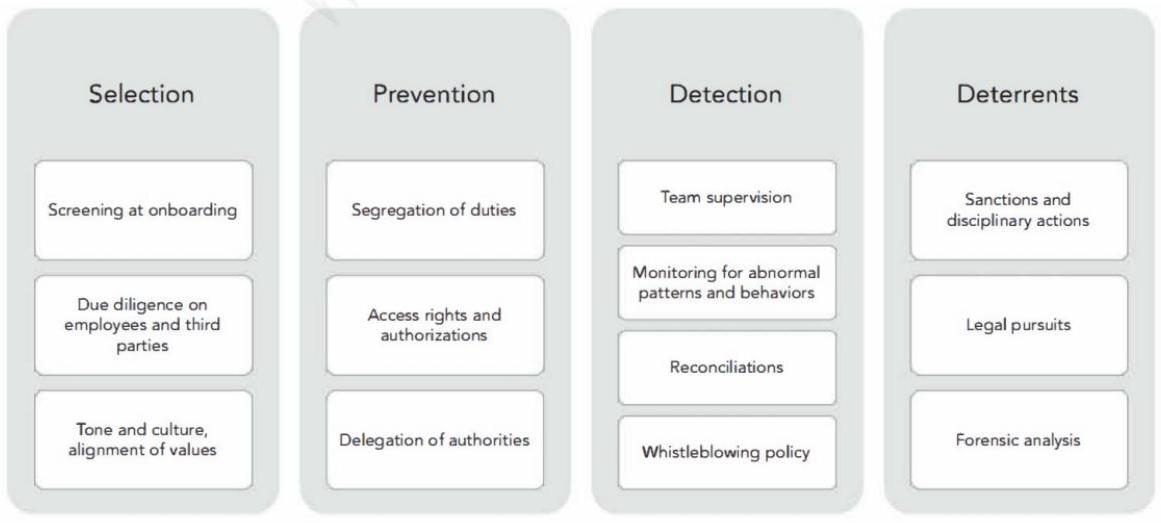
\includegraphics[width=0.8\textwidth]{images/fraud.jpg}
    \caption{fraud}
    \label{fig:label10}
    \end{figure}


\end{itemize}



\subsubsection{AML risk management}
\begin{itemize}
\item The three phases in money laundering are placement, layering, and integration or extraction.
\item Elements of a control framework to manage AML risk:


\begin{figure}[H]
    \centering
    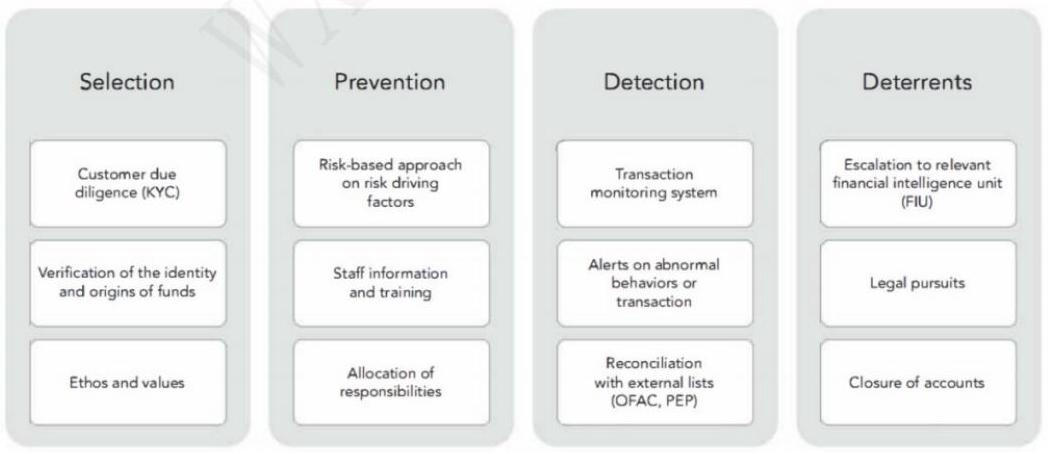
\includegraphics[width=0.8\textwidth]{images/fraud2.jpg}
    \caption{fraud2}
    \label{fig:label11}
    \end{figure}
\end{itemize}



\subsubsection{Case study: USAA }
\begin{itemize}
\item USAA paid \$140 million of fines in AML management failure reached with the Financial Crimes Enforcement Network (FinCEN) and the Office of the Comptroller of the Currency (OCC).
\item The fines were due to a lack of control over AML risk (weak control environment).
\item Regulatory findings and sanctions mean costly AML remediation programs (called lookbacks) in which the bank must review all client files for a specified period, verify client information, file suspicious activity reports and even close suspicious accounts.
\item COVID-19 pandemic makes it more difficult for financial institutions to identify anomalies based on automation of detection prone to false positives, false negatives.
\end{itemize}



\subsection{ Guidance on Managing Outsourcing Risk}


\subsubsection{Risks from the use of service providers }
\begin{itemize}
\item Compliance risks arise when a service provider violates laws/regulations.
\item Concentration risks arise outsourced services are provided by limited service providers or in limited geographic locations.
\item Reputational risks arise bad performance of a service provider causes the public to have negative opinion on financial institution.
\item Country risks arise financial institution engages a foreign service provider, exposing possible risks from the foreign country.
\item Operational risks
\item Legal risks arise when a service provider exposes a financial institution to legal expenses and possible lawsuits.
\end{itemize}



\subsubsection{Elements of effective program to manage outsourcing risk }
\begin{itemize}
\item Risk assessments
\item Due diligence and selection of service providers
\item Contract provisions and considerations
\item Incentive compensation review
\item Oversight and monitoring of service providers
\item Business continuity and contingency plans

\end{itemize}



\subsubsection{Due diligence of service providers}
\begin{itemize}
\item Financial institution should conduct an evaluation of and perform the necessary due diligence for a prospective service provider prior to engaging the service provider. The overall due diligence process includes a review of the service provider with regard to three points.
    \begin{itemize}
    \item Business background, reputation, and strategy
    \item Financial performance and condition
    \item Operations and internal controls
    \end{itemize}
\end{itemize}



\subsubsection{Contract provision }
\begin{itemize}
\item Terms of service agreements should be defined in written contracts that have been reviewed by the financial institution's legal counsel prior to execution. Elements usually include 15 parts.
    \begin{itemize}
    \item Scope: contracts clearly define the rights and responsibilities of each party.
    \item  Cost and compensation: contracts describe the compensation, variable charges, and any fees to be paid for non-recurring items and special requests.
    \item Right to audit: agreements provide for the right of the institution to audit the service provider/access to audit reports. The provision is optionally included.
    \item Establishment and monitoring of performance standards: agreements define measurable performance standards for the services or products being provided.
    \item Confidentiality and security of information: service providers ensure the security and confidentiality of both the institution's information and customer information
    \item Ownership and license: Agreements should address the ownership of any information generated by service providers. Agreements define circumstances under which service providers may use institution property inclusive of data, hardware, software, and intellectual property.
    \item  Indemnification: agreements provide for service provider indemnification of the institutions for any claims against the institutions resulting from the service provider's negligence. 
    \item Default and termination: agreements define events of a contractual default, list of acceptable remedies, and provide opportunities for curing default. Bad performance and nonperformance of duties detected by performance metrics can lead to default and termination.
    \item Dispute resolution: dispute resolution process is to expedite problem resolution and minimize disruption.
    \item Limits on liability: service providers may want to contractually limit their liability.
    \item Insurance: service providers have adequate insurance and provide financial institutions with proof of insurance.
    \item  Customer complaints: agreements specify the responsibilities of both parties related to responding to customer complaints.
    \item  Business resumption and contingency plan of the service provider: the contingency plan is developed by the service provider and reviewed/tested by the financial institution.
    \item Foreign-based service providers: the institutions should consider including choice of law and jurisdictional provisions. This would avoid confusing situations where the foreign laws differ substantially from local laws.
        \begin{itemize}
        \item Banks may apply different standards for local and foreign-based service providers.
        \item Service agreements with foreign-based vendors should always be flexible to allow the laws of home or host country to apply for resolving related disputes. 
        \end{itemize}
    \item Subcontracting: if agreements allow subcontracting, the same contractual provisions should apply to subcontractor. Service providers rather than financial institutions have overall accountability for all services that the service provider and its subcontractors provide
    \end{itemize}
\end{itemize}









\subsection{ Case Study:Third-Party Risk Management}






\subsubsection{Third-party risk}
\begin{itemize}
\item Financial firms contract with third parties for services as a cost-savings approach, outsourcing a wide variety of activities to specialized firms with a competitive advantage in particular systems, processes, and knowledge.
\item While contracting with third-party providers for back-office activities or cloud-based data management may have the potential to reduce process errors or cybersecurity risks, it does not fully mitigate operational risk and increases exposure to "third party risk".
\end{itemize}



\subsubsection{Effective third-party risk management framework }

\begin{figure}[H]
    \centering
    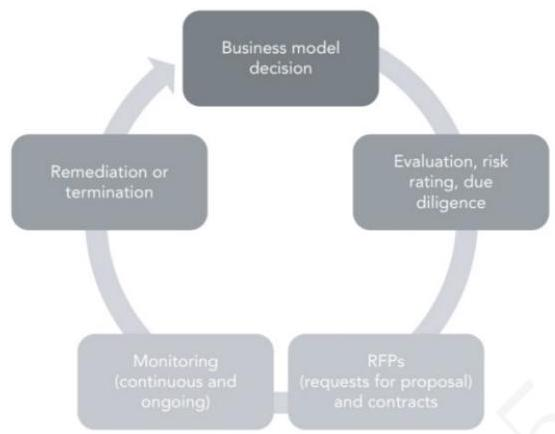
\includegraphics[width=0.8\textwidth]{images/tpframeworks.jpg}
    \caption{tpframeworks}
    \label{fig:label11}
    \end{figure}



\subsubsection{Case study: Capital One data breach}
\begin{itemize}
\item  Case: Federal authorities ultimately arrested a former Amazon Web Services (AWS) cloud services employee for breaking into the bank's server. The former employee of AWS was charged with stealing 140,000 Social Security numbers and 80,000 bank account numbers in the breach.
\item Lessons: The increase in breaches involving cloud databases and services is the result of poor security hygiene
\end{itemize}




\subsubsection{Case study: OCC fines Morgan Stanley }
\begin{itemize}
\item Case: Morgan Stanley received a \$ 60 million fine imposed by the OCC due to failures in the risk management and oversight of vendors in the decommissioning of two wealth management business data servers in 2016.
\item Lessons: The bank did not exercise adequate due diligence in selecting the third-party vendors and did not adequately monitor the vendors'performance.
\end{itemize}





\subsection{ Case study:Investor Protectionand Compliance Risks in Investment Activities}




\subsubsection{MIFID (Markets in Financial Instruments Directive) }

\begin{table}[H]
    \centering
    \caption{Regulations}
    \renewcommand{\arraystretch}{1.5} % 设置行距为1.5
    \begin{tabular}{|p{4cm}|p{10cm}|}
        \hline
        \textbf{Regulations} & \textbf{Description} \\ \hline
        MIFID (2004) & Define regulatory reporting and trade transparency obligation to prevent market abuse and defines the rules on the acceptance of financial instruments for public trading. \\ \hline
        MIFID II (2014) & Alongside the reinforcement of investor protection, MIFID II set out additional requirements on public disclosure of data on trading activity, and on disclosure of transaction data to regulators and supervisors. \\ \hline
    \end{tabular}
\end{table}




\subsubsection{Dodd-Frank}
\begin{itemize}
\item The Investor Protection Act in the USA in 2009.
    \begin{itemize}
    \item Whistleblowers are granted increased protections.
    \item Mandate derivatives need to be traded in clearinghouses.
    \item Aim at ensuring a greater financial stability of the markets.
    \item The Volcker Rule intends to prevent commercial banks from engaging in speculative activities and proprietary trading.
    \item Create Consumer Financial Protection Bureau （CFPB）.
    \end{itemize}


\end{itemize}




\subsubsection{Statistics and record fines cases}
\begin{itemize}
\item The most severe penalty was imposed on UBS for\$ 11.15 billion in 2008 because UBS misrepresented auction rate securities to investors as safe, cash-equivalent products, when in fact they faced increasing liquidity risk.
\item The largest fine for spoofing is held by JP Morgan fined \$ 920 million by the CFTC （Commodity Futures Trading Commission） in September 2020 by US regulators for "spoofing" in the precious metals and US Treasury markets.

\end{itemize}




\subsubsection{FINRA fines Deutsche bank securities}
\begin{itemize}
\item The Financial Industry Regulatory Authority (FINRA) fines Deutsche bank securities, Inc.\$ 2 million for best execution violations.
\item FINRA found that, between 2014 and 2018, Deutsche Bank Securities was routing customer orders to exchanges through its smart order router. This indirect routing of orders created delays of execution in customers'market orders and also caused lower fill rate.
\item Lessons:
    \begin{itemize}
    \item Regulators tend to apply punitive fines such that the penalty more than offsets the benefits accumulated where firms perpetuate non-compliant practices.
    \item The fines are aimed to act as deterrent for further deviations and have a signaling power to peer firms to encourage them to adjust their processes and monitoring practices to ensure compliance.
    \end{itemize}
\end{itemize}




\subsection{ Supervisory Guidanceon Model Risk Management}



\subsubsection{Model}
\begin{itemize}
\item Model refers to a quantitative method, system, or approach that applies statistical, economic, financial, or mathematical theories, techniques, and assumptions to process input data into quantitative estimates.
    \begin{itemize}
    \item A model consists of three components: an information input component; a process component; a reporting
    component.
    \item Models are simplified representations of real-world, focus on particular aspects considered to be most important.
    \end{itemize}
\end{itemize}




\subsubsection{Model risk}
\begin{itemize}
\item Model risk: the potential for adverse consequences from decisions based on incorrect or misused model outputs/reports.
\item Model risk occurs for two reasons:
    \begin{itemize}
    \item Fundamental errors produce inaccurate outputs against the design objective and intended business uses.
    \item The model may be used incorrectly or inappropriately.
    \end{itemize}
\end{itemize}




\subsubsection{Effective framework to manage model risk}
\begin{itemize}
\item  Elements of the framework
    \begin{itemize}
    \item Robust model development, implementation, and use
    \item A sound model validation process
    \item Governance sets an effective framework with defined roles and responsibilities, as well as the authority to restrict model usage.
    \end{itemize}
\end{itemize}




\subsubsection{Elements of the framework一1.development,implementation}
\begin{itemize}
\item At initiation, ensure the model is logical and is on the basis of technically-correct mathematical theories.
\item Then ensure that the data collected and assumptions are robust and relevant for the model.
\item Finally there should be a clear documentation and made clear to users.
\item After developing the model:
    \begin{itemize}
    \item Quantitative aspects: quantitative model testing includes checking the model's accuracy, robust and stable, limitations and the model's assumption/behavior over a range of input values. Testing should be done in both normal and extreme (stressed) market conditions.
    \item Qualitative aspects: Banks should ensure that the development of the more judgmental and qualitative aspects of their models is also sound. 
    \end{itemize}
\end{itemize}




\subsubsection{Elements of the framework-2.validation}

\begin{itemize}
\item Three core elements of effective validation framework 
    \begin{itemize}
    \item  Evaluation of conceptual soundness, including developmental evidence
    \item  Ongoing monitoring , including process verification and benchmarking
    \item  Outcomes analysis, including back-testing
    
    \end{itemize}
\item  Evaluation of conceptual soundness, including developmental evidence
    \begin{itemize}
    \item Carry out overall quality check on the model design and construction.
        \begin{itemize}
        \item Mainly examine the documentation evidence and perform supplemental sensitivity analysis （one variable change） and testing （multiple variables change）.
        \item Qualitative information and judgment in model development should be validated and documented. 
        \end{itemize}
    \end{itemize}
\item Ongoing monitoring
    \begin{itemize}
    \item Once the model comes into play, ongoing monitoring begins. Ongoing monitoring tries to determine whether any changes, additional developments, or replacement should be needed for the model.
    \item Sensitivity analysis and other checks for robustness and stability should likewise be repeated periodically.
    \item Ongoing monitoring should include the analysis of overrides with appropriate documentation.
    \item It includes process verification and benchmarking to confirm the model is implemented as intended.
        \begin{itemize}
        \item Process verification: Ensure data inputs to be error-free and complete. Execute Internal control to ensure computer code can only be altered by authorized staff.
        \item Benchmarking: Compare a model's outputs with other comparable models or inputs with comparable data. Discrepancies should trigger investigation into the sources and degree of the differences. 
        \end{itemize}   
    \end{itemize}
    
\item Outcomes analysis, including back-testing
    \begin{itemize}
    \item Rely on quantitative approaches such as statistical tests and qualitative approaches such as expert judgment.
    \item Outcomes analysis should be conducted on an ongoing basis. Confidence intervals need to be developed based on the model estimates, so that outcomes that are beyond the intervals should be specially focused on and monitored.
    \item Parallel outcomes analysis is based on that models are frequently revised for new information or data.
    \end{itemize}
    
\end{itemize}




\subsubsection{Challenges to an effective validation process}
\begin{itemize}
\item System integration can be a challenge because the model need draw from various sources of data to process huge data, and feeds into multiple data repositories and reporting systems.
\item The widespread use of vendor/third-party products poses unique challenge because the modeling expertise is external to the user and some components may considered proprietary.
\end{itemize}




\subsection{ Case Study: Model Risk and Model Validation}




\subsubsection{Model risk}
\begin{itemize}
\item There are two broad risks an institution can be exposed to due to model risk.
    \begin{itemize}
    \item Execution risk: occurs when a model does not do what it is intended and designed to do.
    \item Conceptual errors: occur when the wrong assumptions or modeling techniques are used in the model.
    \end{itemize}
\end{itemize}




\subsubsection{Model risk management (MRM) function }
\begin{itemize}
\item MRM function sits in the second line of defense and is staffed with experts who are independent of model development.
\item To balance the cost and burden of model validation with the need to ensure that model risk is adequately addressed, MRM functions assign models to different tiers according to the risk they pose to the institution.
\item Highest-tier models will be reviewed in detail, with the validation team performing comprehensive back-testing and assessing the model.
\item High-tier models also undergo more frequent full scope validations, usually every 2 to 3 years.
\item Lower-tier models are subject to a similar process but with the depth and frequency of the various actions tailored to the tier.
\item All models, independently of their tier, undergo an annual review of the environment.
\item Model risk management should be seen as a continuous effort rather than a point-in-time exercise revolving around validations and reviews.
\end{itemize}




\subsubsection{Gaussian Copula and CDO pricing}
\begin{itemize}
\item Case: Correlation assumption is a problem. Banks fail to update the copula model with the new correlation estimates implied by new CDS prices, and continue to price CDOs using the old assumptions.
\item Lessons: The critical responsibility of MRM function is to challenge the assumptions upon which the model relies and ensure that users understand its limitations.

\end{itemize}




\subsubsection{Barclays'acquisition and excel spreadsheet error}
\begin{itemize}
\item Case: Barclays Capital offered to acquire Lehman Brothers' positions after Lehman Brothers filed for bankruptcy, including 179 trading contracts that Barclays did not want to buy. They were hidden rather than deleted. A junior law associate reformatting the Excel file to a PDF makes hidden rows visible again in the PDF file.
\item Lessons: Seemingly simplistic tools or models still need the right review, challenge and controls.
\end{itemize}





\subsubsection{NASA Mars Orbiter}
\begin{itemize}
\item Case: NASA lost a \$125 million Mars orbiter because a Lockheed Martin engineering team used English units of measurement, while the agency's team used the more conventional metric system.
\item Lessons: This is an error in the "assumptions" of the model, the choice of the unit (metric vs imperial). A small subset of these mistakes can result in catastrophic losses (\$125 million).
\end{itemize}


